% Options for packages loaded elsewhere
\PassOptionsToPackage{unicode}{hyperref}
\PassOptionsToPackage{hyphens}{url}
%
\documentclass[
  english,
  man,floatsintext]{apa7}
\usepackage{amsmath,amssymb}
\usepackage{lmodern}
\usepackage{ifxetex,ifluatex}
\ifnum 0\ifxetex 1\fi\ifluatex 1\fi=0 % if pdftex
  \usepackage[T1]{fontenc}
  \usepackage[utf8]{inputenc}
  \usepackage{textcomp} % provide euro and other symbols
\else % if luatex or xetex
  \usepackage{unicode-math}
  \defaultfontfeatures{Scale=MatchLowercase}
  \defaultfontfeatures[\rmfamily]{Ligatures=TeX,Scale=1}
\fi
% Use upquote if available, for straight quotes in verbatim environments
\IfFileExists{upquote.sty}{\usepackage{upquote}}{}
\IfFileExists{microtype.sty}{% use microtype if available
  \usepackage[]{microtype}
  \UseMicrotypeSet[protrusion]{basicmath} % disable protrusion for tt fonts
}{}
\makeatletter
\@ifundefined{KOMAClassName}{% if non-KOMA class
  \IfFileExists{parskip.sty}{%
    \usepackage{parskip}
  }{% else
    \setlength{\parindent}{0pt}
    \setlength{\parskip}{6pt plus 2pt minus 1pt}}
}{% if KOMA class
  \KOMAoptions{parskip=half}}
\makeatother
\usepackage{xcolor}
\IfFileExists{xurl.sty}{\usepackage{xurl}}{} % add URL line breaks if available
\IfFileExists{bookmark.sty}{\usepackage{bookmark}}{\usepackage{hyperref}}
\hypersetup{
  pdftitle={Appendix},
  pdflang={en-EN},
  hidelinks,
  pdfcreator={LaTeX via pandoc}}
\urlstyle{same} % disable monospaced font for URLs
\usepackage{graphicx}
\makeatletter
\def\maxwidth{\ifdim\Gin@nat@width>\linewidth\linewidth\else\Gin@nat@width\fi}
\def\maxheight{\ifdim\Gin@nat@height>\textheight\textheight\else\Gin@nat@height\fi}
\makeatother
% Scale images if necessary, so that they will not overflow the page
% margins by default, and it is still possible to overwrite the defaults
% using explicit options in \includegraphics[width, height, ...]{}
\setkeys{Gin}{width=\maxwidth,height=\maxheight,keepaspectratio}
% Set default figure placement to htbp
\makeatletter
\def\fps@figure{htbp}
\makeatother
\setlength{\emergencystretch}{3em} % prevent overfull lines
\providecommand{\tightlist}{%
  \setlength{\itemsep}{0pt}\setlength{\parskip}{0pt}}
\setcounter{secnumdepth}{5}
% Make \paragraph and \subparagraph free-standing
\ifx\paragraph\undefined\else
  \let\oldparagraph\paragraph
  \renewcommand{\paragraph}[1]{\oldparagraph{#1}\mbox{}}
\fi
\ifx\subparagraph\undefined\else
  \let\oldsubparagraph\subparagraph
  \renewcommand{\subparagraph}[1]{\oldsubparagraph{#1}\mbox{}}
\fi
% Manuscript styling
\usepackage{upgreek}
\captionsetup{font=singlespacing,justification=justified}

% Table formatting
\usepackage{longtable}
\usepackage{lscape}
% \usepackage[counterclockwise]{rotating}   % Landscape page setup for large tables
\usepackage{multirow}		% Table styling
\usepackage{tabularx}		% Control Column width
\usepackage[flushleft]{threeparttable}	% Allows for three part tables with a specified notes section
\usepackage{threeparttablex}            % Lets threeparttable work with longtable

% Create new environments so endfloat can handle them
% \newenvironment{ltable}
%   {\begin{landscape}\begin{center}\begin{threeparttable}}
%   {\end{threeparttable}\end{center}\end{landscape}}
\newenvironment{lltable}{\begin{landscape}\begin{center}\begin{ThreePartTable}}{\end{ThreePartTable}\end{center}\end{landscape}}

% Enables adjusting longtable caption width to table width
% Solution found at http://golatex.de/longtable-mit-caption-so-breit-wie-die-tabelle-t15767.html
\makeatletter
\newcommand\LastLTentrywidth{1em}
\newlength\longtablewidth
\setlength{\longtablewidth}{1in}
\newcommand{\getlongtablewidth}{\begingroup \ifcsname LT@\roman{LT@tables}\endcsname \global\longtablewidth=0pt \renewcommand{\LT@entry}[2]{\global\advance\longtablewidth by ##2\relax\gdef\LastLTentrywidth{##2}}\@nameuse{LT@\roman{LT@tables}} \fi \endgroup}

% \setlength{\parindent}{0.5in}
% \setlength{\parskip}{0pt plus 0pt minus 0pt}

% Overwrite redefinition of paragraph and subparagraph by the default LaTeX template
% See https://github.com/crsh/papaja/issues/292
\makeatletter
\renewcommand{\paragraph}{\@startsection{paragraph}{4}{\parindent}%
  {0\baselineskip \@plus 0.2ex \@minus 0.2ex}%
  {-1em}%
  {\normalfont\normalsize\bfseries\itshape\typesectitle}}

\renewcommand{\subparagraph}[1]{\@startsection{subparagraph}{5}{1em}%
  {0\baselineskip \@plus 0.2ex \@minus 0.2ex}%
  {-\z@\relax}%
  {\normalfont\normalsize\itshape\hspace{\parindent}{#1}\textit{\addperi}}{\relax}}
\makeatother

% \usepackage{etoolbox}
\makeatletter
\patchcmd{\HyOrg@maketitle}
  {\section{\normalfont\normalsize\abstractname}}
  {\section*{\normalfont\normalsize\abstractname}}
  {}{\typeout{Failed to patch abstract.}}
\patchcmd{\HyOrg@maketitle}
  {\section{\protect\normalfont{\@title}}}
  {\section*{\protect\normalfont{\@title}}}
  {}{\typeout{Failed to patch title.}}
\makeatother
\shorttitle{}
\usepackage{csquotes}
\AtBeginEnvironment{tabular}{\doublespacing}
\usepackage[export]{adjustbox}
\ifxetex
  % Load polyglossia as late as possible: uses bidi with RTL langages (e.g. Hebrew, Arabic)
  \usepackage{polyglossia}
  \setmainlanguage[]{english}
\else
  \usepackage[main=english]{babel}
% get rid of language-specific shorthands (see #6817):
\let\LanguageShortHands\languageshorthands
\def\languageshorthands#1{}
\fi
\ifluatex
  \usepackage{selnolig}  % disable illegal ligatures
\fi

\title{Appendix}
\author{\textsuperscript{}}
\date{}


\affiliation{\vspace{0.5cm}\textsuperscript{} }

\begin{document}
\maketitle

\hypertarget{appendix}{%
\section*{Appendix}\label{appendix}}
\addcontentsline{toc}{section}{Appendix}

\setcounter{table}{0}
\renewcommand{\thetable}{A\arabic{table}}

\begin{center}
\begin{ThreePartTable}

\begin{longtable}{llll}\noalign{\getlongtablewidth\global\LTcapwidth=\longtablewidth}
\caption{\label{tab:appendix}Unfamiliar Object Stimuli\smallskip}\\
\toprule
 & \# & Matching keywords & Non-matching keywords\\
\midrule
\endfirsthead
\caption*{\normalfont{Table \ref{tab:appendix} continued}}\\
\toprule
 & \# & Matching keywords & Non-matching keywords\\
\midrule
\endhead
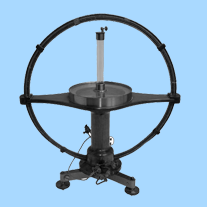
\includegraphics[valign=c, scale=0.19]{../materials/unfamiliar/1.png} & 1 & elektrische Spannung prüfen & Makkaroni formen\\
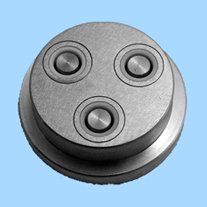
\includegraphics[valign=c, scale=0.19]{../materials/unfamiliar/2.png} & 2 & Makkaroni formen & Kuh vom Zaun abhalten\\
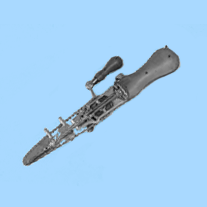
\includegraphics[valign=c, scale=0.19]{../materials/unfamiliar/3.png} & 3 & Knochen sägen & Streckenmaß Sonnenlicht nutzen\\
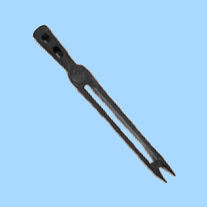
\includegraphics[valign=c, scale=0.19]{../materials/unfamiliar/4.png} & 4 & Unkraut jäten & Uhr mit Wärme betreiben\\
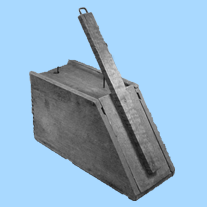
\includegraphics[valign=c, scale=0.19]{../materials/unfamiliar/5.png} & 5 & Mausefalle zuschnappen & Brillenglas zuschneiden\\
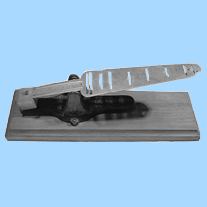
\includegraphics[valign=c, scale=0.19]{../materials/unfamiliar/6.png} & 6 & Goldmünzen wiegen & Farbe vom Fenster abschleifen\\
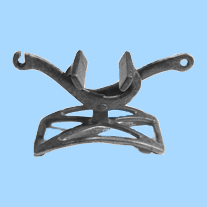
\includegraphics[valign=c, scale=0.19]{../materials/unfamiliar/7.png} & 7 & Knie fixieren & Buchstaben tippen\\
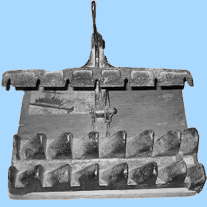
\includegraphics[valign=c, scale=0.19]{../materials/unfamiliar/8.png} & 8 & Eierkarton pressen & Tabak zermahlen\\
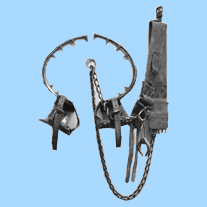
\includegraphics[valign=c, scale=0.19]{../materials/unfamiliar/9.png} & 9 & Baum erklettern & Rotation Ladung erzeugen\\
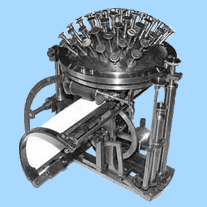
\includegraphics[valign=c, scale=0.19]{../materials/unfamiliar/10.png} & 10 & Buchstaben tippen & Pferdehuf Halt geben\\
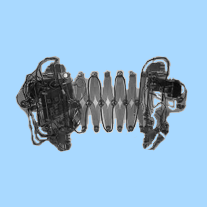
\includegraphics[valign=c, scale=0.19]{../materials/unfamiliar/11.png} & 11 & Akkordeon spielen & Seil schneiden\\
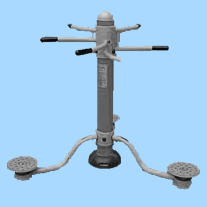
\includegraphics[valign=c, scale=0.19]{../materials/unfamiliar/12.png} & 12 & Körper trainieren & Buch offen halten\\
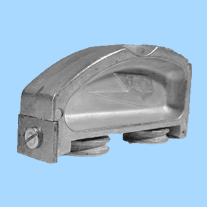
\includegraphics[valign=c, scale=0.19]{../materials/unfamiliar/13.png} & 13 & Farbe vom Fenster abschleifen & von Hand zentrifugieren\\
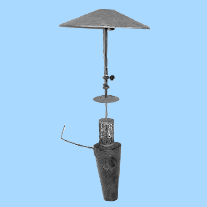
\includegraphics[valign=c, scale=0.19]{../materials/unfamiliar/14.png} & 14 & Außenbereich heizen & Rasierklinge schärfen\\
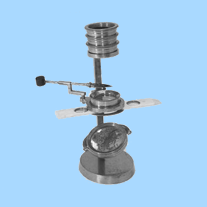
\includegraphics[valign=c, scale=0.19]{../materials/unfamiliar/15.png} & 15 & Pflanzenteile vergrößern & Katzenklo sich selbst reinigen\\
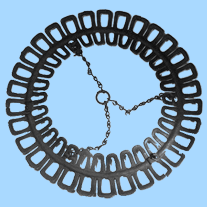
\includegraphics[valign=c, scale=0.19]{../materials/unfamiliar/16.png} & 16 & Krawatten aufhängen & Zeichnungen vermessen\\
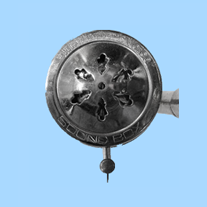
\includegraphics[valign=c, scale=0.19]{../materials/unfamiliar/17.png} & 17 & Schallplatte abtasten & Ball katapultieren\\
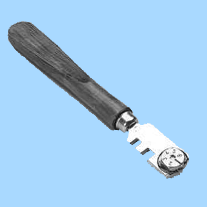
\includegraphics[valign=c, scale=0.19]{../materials/unfamiliar/18.png} & 18 & Glas schneiden & Eier wiegen\\
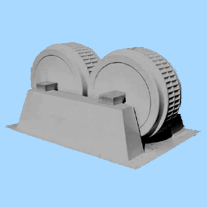
\includegraphics[valign=c, scale=0.19]{../materials/unfamiliar/19.png} & 19 & Briketts pressen & Narkosemittel abgeben\\
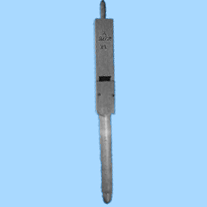
\includegraphics[valign=c, scale=0.19]{../materials/unfamiliar/20.png} & 20 & Orgelton erzeugen & Bandage rollen\\
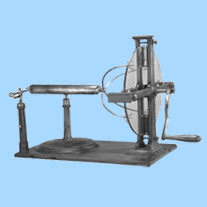
\includegraphics[valign=c, scale=0.19]{../materials/unfamiliar/21.png} & 21 & Spannung erzeugen & Fußstütze reiten\\
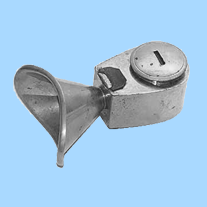
\includegraphics[valign=c, scale=0.19]{../materials/unfamiliar/22.png} & 22 & Narkosemittel abgeben & Nüsse aufbrechen\\
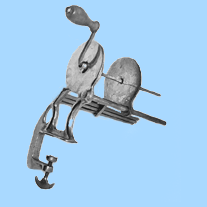
\includegraphics[valign=c, scale=0.19]{../materials/unfamiliar/23.png} & 23 & Bandage rollen & Schnee rodeln\\
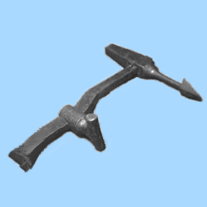
\includegraphics[valign=c, scale=0.19]{../materials/unfamiliar/24.png} & 24 & Weinfass Loch einschlagen & Tier einfangen\\
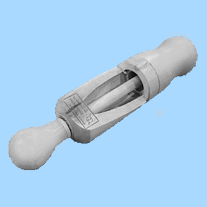
\includegraphics[valign=c, scale=0.19]{../materials/unfamiliar/25.png} & 25 & Flaschenkorken einführen & Pferd im Moor laufen\\
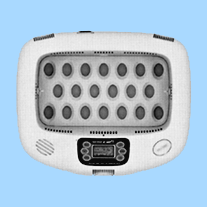
\includegraphics[valign=c, scale=0.19]{../materials/unfamiliar/26.png} & 26 & Automat Eier ausbrüten & Windgeschwindigkeit messen\\
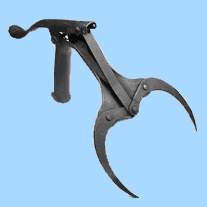
\includegraphics[valign=c, scale=0.19]{../materials/unfamiliar/27.png} & 27 & Korngarbe greifen & Treibhaus heizen\\
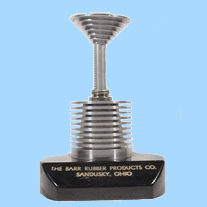
\includegraphics[valign=c, scale=0.19]{../materials/unfamiliar/28.png} & 28 & Brief wiegen & Korngarbe greifen\\
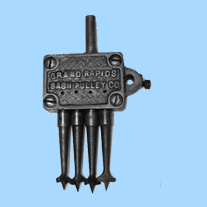
\includegraphics[valign=c, scale=0.19]{../materials/unfamiliar/29.png} & 29 & Löcher bohren & Sonnenlicht Intensität messen\\
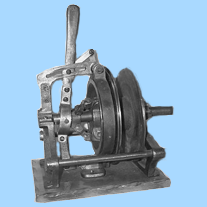
\includegraphics[valign=c, scale=0.19]{../materials/unfamiliar/30.png} & 30 & Angelschnur kurbeln & Glaskörper musizieren\\
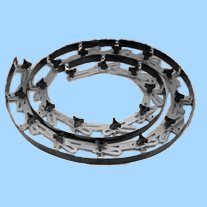
\includegraphics[valign=c, scale=0.19]{../materials/unfamiliar/31.png} & 31 & Kurven malen & Nussöl pressen\\
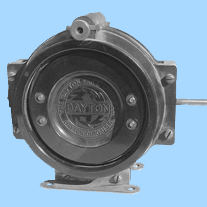
\includegraphics[valign=c, scale=0.19]{../materials/unfamiliar/32.png} & 32 & Radiofrequenz einstellen & Erektion helfen\\
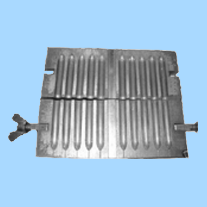
\includegraphics[valign=c, scale=0.19]{../materials/unfamiliar/33.png} & 33 & Zäpfchen pressen & Unkraut jäten\\
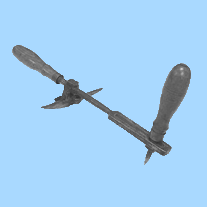
\includegraphics[valign=c, scale=0.19]{../materials/unfamiliar/34.png} & 34 & Fass öffnen & Pflanzenteile vergrößern\\
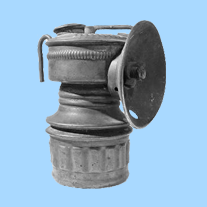
\includegraphics[valign=c, scale=0.19]{../materials/unfamiliar/35.png} & 35 & Bergbaustollen beleuchten & Knie fixieren\\
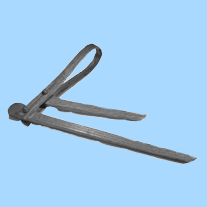
\includegraphics[valign=c, scale=0.19]{../materials/unfamiliar/36.png} & 36 & Kuh vom Zaun abhalten & Radiofrequenz einstellen\\
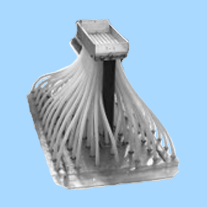
\includegraphics[valign=c, scale=0.19]{../materials/unfamiliar/37.png} & 37 & Saatgut gleichmäßig aussäen & Fass öffnen\\
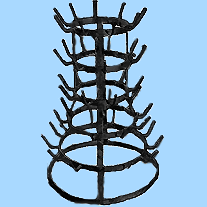
\includegraphics[valign=c, scale=0.19]{../materials/unfamiliar/38.png} & 38 & Flaschen trocknen & Bleistift anspitzen\\
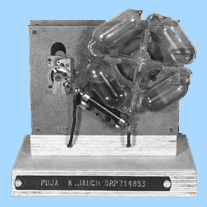
\includegraphics[valign=c, scale=0.19]{../materials/unfamiliar/39.png} & 39 & Uhr mit Wärme betreiben & Körper untersuchen\\
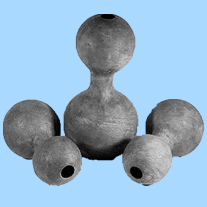
\includegraphics[valign=c, scale=0.19]{../materials/unfamiliar/40.png} & 40 & Tonpott trommeln & Piano stimmen\\
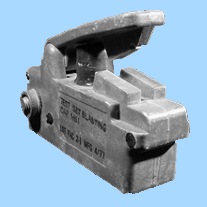
\includegraphics[valign=c, scale=0.19]{../materials/unfamiliar/41.png} & 41 & Sprengstoffexplosion auslösen & Fisch wiegen\\
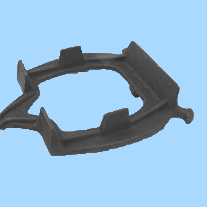
\includegraphics[valign=c, scale=0.19]{../materials/unfamiliar/42.png} & 42 & Pferdehuf Halt geben & Zäpfchen pressen\\
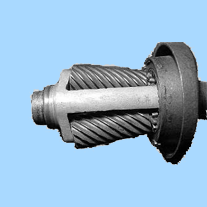
\includegraphics[valign=c, scale=0.19]{../materials/unfamiliar/43.png} & 43 & Bleistift anspitzen & Angel Köder markieren\\
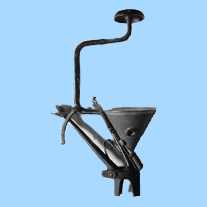
\includegraphics[valign=c, scale=0.19]{../materials/unfamiliar/44.png} & 44 & Nussöl pressen & Zeichen einbrennen\\
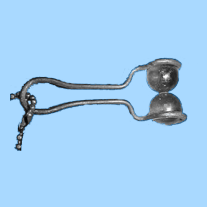
\includegraphics[valign=c, scale=0.19]{../materials/unfamiliar/45.png} & 45 & Rasierklinge schärfen & Kurven malen\\
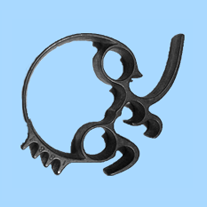
\includegraphics[valign=c, scale=0.19]{../materials/unfamiliar/46.png} & 46 & heiße Platten anheben & Kleidung im Eimer waschen\\
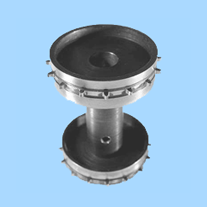
\includegraphics[valign=c, scale=0.19]{../materials/unfamiliar/47.png} & 47 & Film aufspulen & Mund offen halten\\
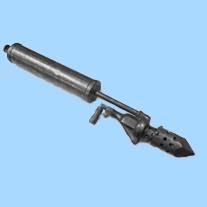
\includegraphics[valign=c, scale=0.19]{../materials/unfamiliar/48.png} & 48 & Waffe entflammen & Uhrzeit anzeigen\\
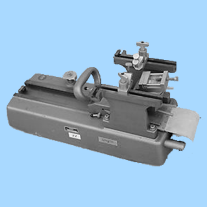
\includegraphics[valign=c, scale=0.19]{../materials/unfamiliar/49.png} & 49 & Mikroskop-Proben schneiden & heiße Platten anheben\\
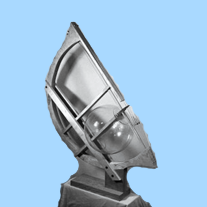
\includegraphics[valign=c, scale=0.19]{../materials/unfamiliar/50.png} & 50 & Glaskörper musizieren & Kork flach pressen\\
\includegraphics[valign=c, scale=0.19]{../materials/unfamiliar/51.png} & 51 & Dampf zerstäuben & Buch binden\\
\includegraphics[valign=c, scale=0.19]{../materials/unfamiliar/52.png} & 52 & Mandeln operieren & Film aufspulen\\
\includegraphics[valign=c, scale=0.19]{../materials/unfamiliar/53.png} & 53 & Toastbrot rösten & Autobatterie Spannung testen\\
\includegraphics[valign=c, scale=0.19]{../materials/unfamiliar/54.png} & 54 & Fußstütze reiten & Stromstärke messen\\
\includegraphics[valign=c, scale=0.19]{../materials/unfamiliar/55.png} & 55 & Türgelenk Feuer überstehen & Botschaft telegrafieren\\
\includegraphics[valign=c, scale=0.19]{../materials/unfamiliar/56.png} & 56 & Schnee rodeln & Dampf zerstäuben\\
\includegraphics[valign=c, scale=0.19]{../materials/unfamiliar/57.png} & 57 & Nüsse aufbrechen & Ziegelsteine formen\\
\includegraphics[valign=c, scale=0.19]{../materials/unfamiliar/58.png} & 58 & Radiergummi mit Strom betreiben & Münzen aufbewahren\\
\includegraphics[valign=c, scale=0.19]{../materials/unfamiliar/59.png} & 59 & Treibhaus heizen & Messer schleifen\\
\includegraphics[valign=c, scale=0.19]{../materials/unfamiliar/60.png} & 60 & Botschaft telegrafieren & Toastbrot rösten\\
\includegraphics[valign=c, scale=0.19]{../materials/unfamiliar/61.png} & 61 & Angel Köder markieren & Baum erklettern\\
\includegraphics[valign=c, scale=0.19]{../materials/unfamiliar/62.png} & 62 & Katzenklo sich selbst reinigen & Tankfüllstand messen\\
\includegraphics[valign=c, scale=0.19]{../materials/unfamiliar/63.png} & 63 & Körper untersuchen & Schuhe auf Eis laufen\\
\includegraphics[valign=c, scale=0.19]{../materials/unfamiliar/64.png} & 64 & Brillenglas zuschneiden & Saatgut gleichmäßig aussäen\\
\includegraphics[valign=c, scale=0.19]{../materials/unfamiliar/65.png} & 65 & Draht wickeln & Bergbaustollen beleuchten\\
\includegraphics[valign=c, scale=0.19]{../materials/unfamiliar/66.png} & 66 & Buch offen halten & Sprengstoffexplosion auslösen\\
\includegraphics[valign=c, scale=0.19]{../materials/unfamiliar/67.png} & 67 & Feldanbau häckseln & Draht wickeln\\
\includegraphics[valign=c, scale=0.19]{../materials/unfamiliar/68.png} & 68 & Schnurlot absenken & Korken formen\\
\includegraphics[valign=c, scale=0.19]{../materials/unfamiliar/69.png} & 69 & Sternenbilder vermessen & Schnurlot absenken\\
\includegraphics[valign=c, scale=0.19]{../materials/unfamiliar/70.png} & 70 & Nachricht morsen & Feldanbau häckseln\\
\includegraphics[valign=c, scale=0.19]{../materials/unfamiliar/71.png} & 71 & Musikgerät stampfen & Goldmünzen wiegen\\
\includegraphics[valign=c, scale=0.19]{../materials/unfamiliar/72.png} & 72 & Schuhe auf Eis laufen & Geschwindigkeit ermitteln\\
\includegraphics[valign=c, scale=0.19]{../materials/unfamiliar/73.png} & 73 & Geschwindigkeit ermitteln & Mausefalle zuschnappen\\
\includegraphics[valign=c, scale=0.19]{../materials/unfamiliar/74.png} & 74 & Zeichen einbrennen & Luftdruck messen\\
\includegraphics[valign=c, scale=0.19]{../materials/unfamiliar/75.png} & 75 & Tabak zermahlen & Flaschen trocknen\\
\includegraphics[valign=c, scale=0.19]{../materials/unfamiliar/76.png} & 76 & Stromstärke messen & Mandeln operieren\\
\includegraphics[valign=c, scale=0.19]{../materials/unfamiliar/77.png} & 77 & Tier einfangen & Maiskolben entkörnen\\
\includegraphics[valign=c, scale=0.19]{../materials/unfamiliar/78.png} & 78 & Messer schleifen & Schritte vergrößern\\
\includegraphics[valign=c, scale=0.19]{../materials/unfamiliar/79.png} & 79 & Leierkasten klingen & Fass anheben\\
\includegraphics[valign=c, scale=0.19]{../materials/unfamiliar/80.png} & 80 & Buch binden & Löcher bohren\\
\includegraphics[valign=c, scale=0.19]{../materials/unfamiliar/81.png} & 81 & Kork flach pressen & Elektroschock spielen\\
\includegraphics[valign=c, scale=0.19]{../materials/unfamiliar/82.png} & 82 & Tabletten zerteilen & Blumentopf sich selbst wässern\\
\includegraphics[valign=c, scale=0.19]{../materials/unfamiliar/83.png} & 83 & Fass anheben & Mikroskop-Proben schneiden\\
\includegraphics[valign=c, scale=0.19]{../materials/unfamiliar/84.png} & 84 & Pferd im Moor laufen & Luft abpumpen\\
\includegraphics[valign=c, scale=0.19]{../materials/unfamiliar/85.png} & 85 & altes Ritual hacken & Spannung erzeugen\\
\includegraphics[valign=c, scale=0.19]{../materials/unfamiliar/86.png} & 86 & Kleidung im Eimer waschen & Türgelenk Feuer überstehen\\
\includegraphics[valign=c, scale=0.19]{../materials/unfamiliar/87.png} & 87 & Maiskolben entkörnen & Brief wiegen\\
\includegraphics[valign=c, scale=0.19]{../materials/unfamiliar/88.png} & 88 & Ball katapultieren & Radiergummi mit Strom betreiben\\
\includegraphics[valign=c, scale=0.19]{../materials/unfamiliar/89.png} & 89 & Zeichnungen vermessen & Brenner löten\\
\includegraphics[valign=c, scale=0.19]{../materials/unfamiliar/90.png} & 90 & Elektroschock spielen & Weinfass Loch einschlagen\\
\includegraphics[valign=c, scale=0.19]{../materials/unfamiliar/91.png} & 91 & Lieferungen abzählen & Außenbereich heizen\\
\includegraphics[valign=c, scale=0.19]{../materials/unfamiliar/92.png} & 92 & Rotation Ladung erzeugen & Musikgerät stampfen\\
\includegraphics[valign=c, scale=0.19]{../materials/unfamiliar/93.png} & 93 & Herz durch Maschine ersetzen & Kerzen löschen\\
\includegraphics[valign=c, scale=0.19]{../materials/unfamiliar/94.png} & 94 & Seil schneiden & Akkordeon spielen\\
\includegraphics[valign=c, scale=0.19]{../materials/unfamiliar/95.png} & 95 & Fisch wiegen & Herz durch Maschine ersetzen\\
\includegraphics[valign=c, scale=0.19]{../materials/unfamiliar/96.png} & 96 & Kerzen löschen & Körper trainieren\\
\includegraphics[valign=c, scale=0.19]{../materials/unfamiliar/97.png} & 97 & Korken formen & Sternenbilder vermessen\\
\includegraphics[valign=c, scale=0.19]{../materials/unfamiliar/98.png} & 98 & Erektion helfen & Waffe werfen\\
\includegraphics[valign=c, scale=0.19]{../materials/unfamiliar/99.png} & 99 & Streckenmaß Sonnenlicht nutzen & Kartoffeln stampfen\\
\includegraphics[valign=c, scale=0.19]{../materials/unfamiliar/100.png} & 100 & Luftdruck messen & Knochen sägen\\
\includegraphics[valign=c, scale=0.19]{../materials/unfamiliar/101.png} & 101 & Piano stimmen & Eierkarton pressen\\
\includegraphics[valign=c, scale=0.19]{../materials/unfamiliar/102.png} & 102 & von Hand zentrifugieren & Lieferungen abzählen\\
\includegraphics[valign=c, scale=0.19]{../materials/unfamiliar/103.png} & 103 & Kartoffeln stampfen & Nachricht morsen\\
\includegraphics[valign=c, scale=0.19]{../materials/unfamiliar/104.png} & 104 & Waffe werfen & elektrische Spannung prüfen\\
\includegraphics[valign=c, scale=0.19]{../materials/unfamiliar/105.png} & 105 & Tankfüllstand messen & Tonpott trommeln\\
\includegraphics[valign=c, scale=0.19]{../materials/unfamiliar/106.png} & 106 & Uhrzeit anzeigen & altes Ritual hacken\\
\includegraphics[valign=c, scale=0.19]{../materials/unfamiliar/107.png} & 107 & Windgeschwindigkeit messen & Waffe entflammen\\
\includegraphics[valign=c, scale=0.19]{../materials/unfamiliar/108.png} & 108 & Schlüsselloch stanzen & Automat Eier ausbrüten\\
\includegraphics[valign=c, scale=0.19]{../materials/unfamiliar/109.png} & 109 & Ziegelsteine formen & Schallplatte abtasten\\
\includegraphics[valign=c, scale=0.19]{../materials/unfamiliar/110.png} & 110 & Becher Schall auffangen & Schlüsselloch stanzen\\
\includegraphics[valign=c, scale=0.19]{../materials/unfamiliar/111.png} & 111 & Luft abpumpen & Briketts pressen\\
\includegraphics[valign=c, scale=0.19]{../materials/unfamiliar/112.png} & 112 & Mund offen halten & Orgelton erzeugen\\
\includegraphics[valign=c, scale=0.19]{../materials/unfamiliar/113.png} & 113 & Autobatterie Spannung testen & Becher Schall auffangen\\
\includegraphics[valign=c, scale=0.19]{../materials/unfamiliar/114.png} & 114 & Sonnenlicht Intensität messen & Krawatten aufhängen\\
\includegraphics[valign=c, scale=0.19]{../materials/unfamiliar/115.png} & 115 & Kutschrad anschließen & Angelschnur kurbeln\\
\includegraphics[valign=c, scale=0.19]{../materials/unfamiliar/116.png} & 116 & Eier wiegen & Leierkasten klingen\\
\includegraphics[valign=c, scale=0.19]{../materials/unfamiliar/117.png} & 117 & Blumentopf sich selbst wässern & Glas schneiden\\
\includegraphics[valign=c, scale=0.19]{../materials/unfamiliar/118.png} & 118 & Schritte vergrößern & Tabletten zerteilen\\
\includegraphics[valign=c, scale=0.19]{../materials/unfamiliar/119.png} & 119 & Münzen aufbewahren & Kutschrad anschließen\\
\includegraphics[valign=c, scale=0.19]{../materials/unfamiliar/120.png} & 120 & Brenner löten & Flaschenkorken einführen einführen\\
\bottomrule
\end{longtable}

\end{ThreePartTable}
\end{center}


\end{document}
